% !TEX TS-program = pdflatex
% !TEX encoding = UTF-8 Unicode

% This is a simple template for a LaTeX document using the "article" class.
% See "book", "report", "letter" for other types of document.

\documentclass[11pt]{article} % use larger type; default would be 10pt

\usepackage[utf8]{inputenc} % set input encoding (not needed with XeLaTeX)

%%% Examples of Article customizations
% These packages are optional, depending whether you want the features they provide.
% See the LaTeX Companion or other references for full information.

%%% PAGE DIMENSIONS
\usepackage{geometry} % to change the page dimensions
\usepackage{graphicx}
\geometry{a4paper} % or letterpaper (US) or a5paper or....
% \geometry{margin=2in} % for example, change the margins to 2 inches all round
% \geometry{landscape} % set up the page for landscape
%   read geometry.pdf for detailed page layout information

\usepackage{graphicx} % support the \includegraphics command and options

% \usepackage[parfill]{parskip} % Activate to begin paragraphs with an empty line rather than an indent

%%% PACKAGES
\usepackage{booktabs} % for much better looking tables
\usepackage{array} % for better arrays (eg matrices) in maths
\usepackage{paralist} % very flexible & customisable lists (eg. enumerate/itemize, etc.)
\usepackage{verbatim} % adds environment for commenting out blocks of text & for better verbatim
\usepackage{subfig} % make it possible to include more than one captioned figure/table in a single float
% These packages are all incorporated in the memoir class to one degree or another...

%%% HEADERS & FOOTERS
\usepackage{fancyhdr} % This should be set AFTER setting up the page geometry
\pagestyle{fancy} % options: empty , plain , fancy
%\setlength{\headheight}{-25pt}
\renewcommand{\headrulewidth}{0pt} % customise the layout...
\lhead{}\chead{}\rhead{}
\lfoot{}\cfoot{\thepage}\rfoot{}

%%% SECTION TITLE APPEARANCE
\usepackage{sectsty}
\allsectionsfont{\sffamily\mdseries\upshape} % (See the fntguide.pdf for font help)
% (This matches ConTeXt defaults)

%%% ToC (table of contents) APPEARANCE
\usepackage[nottoc,notlof,notlot]{tocbibind} % Put the bibliography in the ToC
\usepackage[titles,subfigure]{tocloft} % Alter the style of the Table of Contents
\renewcommand{\cftsecfont}{\rmfamily\mdseries\upshape}
\renewcommand{\cftsecpagefont}{\rmfamily\mdseries\upshape} % No bold!

%%% END Article customizations

%%% The "real" document content comes below...

\title{Homework 2}
\author{Maksim Levental}
%\date{} % Activate to display a given date or no date (if empty),
         % otherwise the current date is printed 

\usepackage{listings}
\usepackage{color}

\definecolor{dkgreen}{rgb}{0,0.6,0}
\definecolor{gray}{rgb}{0.5,0.5,0.5}
\definecolor{mauve}{rgb}{0.58,0,0.82}

\lstset{frame=tb,
  language=C++,
  aboveskip=3mm,
  belowskip=3mm,
  showstringspaces=false,
  columns=flexible,
  basicstyle={\small\ttfamily},
  numbers=none,
  numberstyle=\tiny\color{gray},
  keywordstyle=\color{blue},
  commentstyle=\color{dkgreen},
  stringstyle=\color{mauve},
  breaklines=false,
  breakatwhitespace=false,
  tabsize=3,
  frame=0
}

\begin{document}
\maketitle

\section*{Problem 1}
\subsection*{Uniprocessor Case}

\textbf{i}) Under user-level thread management none of the states are possible. In user-level thread management if any of the threads in a process are blocked then the whole process becomes blocked. So all the processes that have one thread blocked would infact have all threads blocked. \bigskip

\noindent \textbf{ii}) Under kernel level thread management all of the states are possible except s5 because it's a uniprocessor system and hence two threads can't run simultaneously. Furthermore the possible state transitions:\bigskip

\noindent s1 \overrightarrow{} s4 is possible supposing the scheduler pre-empts s1. s4 would then replace s1 as the running thread because it's in the ready state.
s4  \overrightarrow{} s1 is possible for similar reasons as above.\bigskip

\noindent s2 \overrightarrow{} s3 is possible supposing Thread 2 blocks waiting for I/O. If that happens Thread 3 will then start running because it was ready.\bigskip

\noindent \textbf{iii}) Under hybrid thread management s1, s3, and s4 are possible. s2 is impossible because  Thread 1 being blocked would block both Thread 1 and Thread 2 and s5 is impossible because Thread 1 and Thread 2 can't run simultaneously on a uniprocessor system. Furthermore the possible state transitions:\bigskip

\noindent s1 \overrightarrow{} s4 and s4 \overrightarrow{} s1 is possible supposing the scheduler pre-empts s1, or s4. s4 would then replace s1 as the running thread because it's in the ready state. Similarly for the inverse.\bigskip

\noindent s1 \overrightarrow{} s3 is possible if Thread 2 blocks for I/O. Then the whole kernel thread associated with those 2 user threads blocks and Thread 3 unblocks and immediately runs because no other kernel level threads exist to pre-empt it. 
s3 \overrightarrow{} s1, the inverse of above, is possible if Thread 3 blocks for I/O.  When that happens the kernel level thread associated with Threads 1 and 2 wakes and one of the user level threads runs and one becomes ready.\bigskip

\noindent s3  \overleftarrow{}\overrightarrow{} s4 is similar to the case for s1  \overleftarrow{}\overrightarrow{} s3.

\subsection*{Multiprocessor case}

\noindent \textbf{i}) Same as in the uniprocessor case. Because threads are user level managed none of the states are possible, even s5, because the kernel sees only one process.
\bigskip

\noindent \textbf{ii}) Same as in the uniprocessor case except that s5 is now possible because two threads can in fact run simultaneously. Possible \textbf{new} (in addition to the ones already listed for the uniprocessor case) transitions now include:

\bigskip
\noindent s4 \overrightarrow{} s5 if Thread 3 becomes unblocked and Thread 2 gets put on its own processor. 
\bigskip

\noindent s1 \overrightarrow{} s5 if Thread 3 becomes unblocked and Thread 1 gets put on its own processor.
\bigskip

\noindent \textbf{iii}) Same as in the uniprocessor case. No new state transitions are allowed because Thread 1 and Thread 2 share one kernel level thread.
\section*{Problem 2}
This scheme for mutual exclusion would fail and here is the counterexample. Imagine there are two threads being managed by the kernel. Without loss of generality suppose Thread 1 begins first. It continues onto the while loop conditional check and bypasses it, since OCCUPIED is set to \textbf{false}. Finally it is pre-empted and, immediately before setting OCCUPIED to \textbf{true}. Thread 2 then runs, proceeds through the while conditional check and also bypasses. It then continues onto the critical region and is pre-empted. Thread 1 wakes again and now both Thread 1 and Thread 2 are both inside the critical region.
\section*{Problem 3}

a) Feasible.
\bigskip

\begin{tabular}{ l l l }
  Thread & mutex.count & mutex.waitingList \\
  T1.1 & 0 & 0 \\
  T1.2 & 0 & 0 \\
  T2.1 & 0 & 1 \\
  T1.3 & 1 & 1 \\
  T2.2 & 0 & 0 \\
  T2.3 & 1 & 0 \\
\end{tabular}
\bigskip

Between T1.3 and T2.2 Thread 2 leaves the waiting list and reduces the count simultaneously.
\bigskip
\bigskip
\bigskip
\bigskip\bigskip\bigskip\bigskip\bigskip\bigskip

\noindent b) Infeasible.
\bigskip

\begin{tabular}{ l l l }
  Thread & mutex.count & mutex.waitingList \\
  T2.1 & 0 & 0 \\
  T2.2 & 0 & 0 \\
  T1.1 & 0 & 1 \\
  T1.2 & 0 & 1 \\
\end{tabular}
\bigskip

Thread 1 would not be able to proceed past executing the down operation on the mutex so this order of execution is not possible.
\bigskip

\noindent c) Feasible.
\bigskip

\begin{tabular}{ l l l }
  Thread & mutex.count & mutex.waitingList \\
  T1.1 & 0 & 0 \\
  T2.1 & 0 & 1 \\
  T1.2 & 0 & 1 \\
  T1.3 & 1 & 1 \\
  T2.2 & 0 & 0 \\
  T2.3 & 1 & 0 \\
\end{tabular}
\bigskip

\noindent d) Feasible.
\bigskip

\begin{tabular}{ l l l }
  Thread & mutex.count & mutex.waitingList \\
  T1.1 & 0 & 0 \\
  T1.2 & 0 & 0 \\
  T1.3 & 1 & 0 \\
  T2.1 & 0 & 0 \\
  T2.2 & 0 & 0 \\
  T2.3 & 0 & 0 \\
\end{tabular}
\bigskip


\section*{Problem 4}
A blackshading indicates running time. A grey shading indicates blocking time.

\bigskip

\noindent Total time taken to run in scheduling scenario one for process one is 20 milliseconds. Total time taken to run in scheduling scenario one for process two is 26 milliseconds. 

\bigskip

\noindent 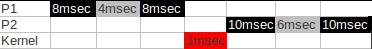
\includegraphics{one.png}

\bigskip\bigskip

\noindent Total time taken to run in scheduling scenario two for process one is 16 milliseconds. Total time taken to run in scheduling scenario two for process two is 20 milliseconds.

\bigskip

\noindent \scalebox{.5}{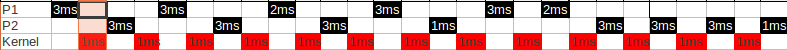
\includegraphics{two.png}}

\bigskip

\noindent Total time taken to run in scheduling scenario three for process one is 20 milliseconds. Total time taken to run in scheduling scenario three for process two is 26 milliseconds.

\bigskip

\noindent 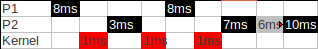
\includegraphics{three.png}

\bigskip



\section*{Problem 5}

This mechanism would not work on a system with priority scheduling. Here is a counterexample that creates \textbf{deadlock}:
\bigskip

\noindent Imagine 3 threads Thread 1 Thread 2 and Thread 3, with consecutively higher scheduling priorities. The process begins running and Thread 2 and Thread 3 block outside of the MUTEXLOCK. Thread 1 enters the MUTEXLOCK. LOCK = 0 because no one is in the MUTEXLOCK already so REGISTER is set to 0 and and LOCK is set to 1. Thread 1 then exits MUTEXLOCK, begins running critical code, and is finally pre-empted because Thread 2 unblocks. Thread 2 enters the MUTEXLOCK but LOCK is 1, because Thread 1 was pre-empted before MUTEUNLOCK, so Thread 2 sets register to 1 and busy waits because of the JNE instruction. Finally Thread 2 is pre-empted by Thread 3 when it becomes unblocked, not Thread 1 because it is of lower priority than Thread 3, and Thread 2 goes into a ready state. But the same thing that occurred with Thread 2 occurs with Thread 3. It busy waits until its quantum expires and then Thread 2 runs, because it is higher priority than Thread 1. And it again busy waits until its quantum expires. This process repeats because Thread 1 can never leave the critical region and set LOCK back to 0. Hence deadlock. 

\end{document}
